\section{Engineered cloth folding pipelines} \label{sec:lit_cloth_folding_pipelines}
%  wat is het doel van deze subsectie?  = Inzicht verschaffen in hoe "klassieke" pipelines het probleem opdelen (is al geschreven :)) en hoe ze die problemen typisch aanpakken. Doel is dat lezer hieruit kan afleiden dat dat wel cool is maar: traag, error accumulation, geen knowledge reuse etc. 
% Cloth folding pipelines (houvast = Sanchez2018, Matas, Douman2016)
A high-level categorization of cloth tasks are \emph{sensing} of material properties, \emph{grasping} a single clothing item in a clutter environment and task-specific \emph{manipulation} applications. Specific applications dealing with manipulation of cloth are folding clothing items, hanging cloth on a rod and bedsheet folding among others. In this dissertation, we focus on the application of cloth folding. A complete cloth folding pipeline typically consists of the following subtasks: (1) grasping an isolated garment, (2) bringing it into a folded configuration and (3) stacking it on top of other folded garments. The second step in this process is often subdivided into unfolding, flattening and folding. Most of the work in robotic cloth folding deal with a single subtask instead of providing solutions to the complete pipeline. Two notable exceptions that consider the whole robotic folding pipeline is the work of~\textcite{Doumanoglou2016,Maitin2010}, which is discussed at the end of this section.
% TODO: add figure of robotic folding pipeline
\tikzstyle{block} = [rectangle, draw, fill=blue!15, text width=8.0em, minimum height=1cm, text centered, rounded corners]
\begin{figure}[htbp!]
    \centering
    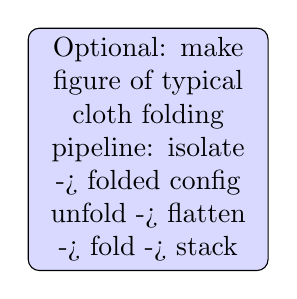
\begin{tikzpicture}[auto, align=center]]
        \node (mock) [block] {Optional: make figure of typical cloth folding pipeline: isolate -> folded config {unfold -> flatten -> fold} -> stack};
    \end{tikzpicture}
    \caption{Optional figure.}
\end{figure}

An evident solution for cloth folding is to use specialized hardware in a constrained environment.~\Textcite{Nair2013} propose an actuated flipfold\footnote{A flipfold is a device consisting of four panels joined by hinges. The four panels lineup with the two sleeves, top-center and bottom-center of the shirt respectively. The hinges allow the panels to rotate inwards. This movement takes the cloth with it and as such makes the folds.} that automates folding of shirts. More complex commercially available products exists such as the FoldiMate\footnote{\url{https://foldimate.com/}}. However, such products do not generalize towards general cloth folding, do not leverage general-purpose robotic hardware and have proven difficult to bring commercially available\footnote{FoldiMate has been in prototype development for nine years at time of writing.}. This is why most research consider the use of general-purpose robot arms, possibly with dedicated gripper and instrumentation, as elaborated in Section~\ref{sec:lit_instrumentation}.

Much of the literature around cloth folding has resolved around solving subtasks of the folding pipeline. In the following subsections, we provide a summary of important work concerning each of the subtasks and describe two important works that consider the complete folding pipeline.

\subsection{Grasping}
Grasping a piece of cloth requires isolating a single piece of garment from a pile of clothing articles and making sure that one functional piece is grasped. In~\autocite{Ramisa2012}, this is done by grasping shirts via the collar. Visual servoing is used with preprocessed features on depth data. Their method achieves a grasping success rate of $70\%$. However, the performance drops to $30\%$ when other types of garments are present on the table. ~\autocite{Monso2012} separate all clothing articles with a robot manipulator. Occlusion of clothing articles leads to uncertainty of the state estimation. They model this explicitly by training a \acrshort{POMDP} for the cloth state estimation.

\subsection{Pose estimation}
After grasping a clothing article, pose estimation is usually done such that the type and configuration of the cloth can be brought into an unfolded state, ready for folding. Garment pose estimation has been done by matching video images to simulation models~\autocite{Kita2002}, using machine learning models~\autocite{Li2014, li2014volum} or instrumentation via fiducial markers~\autocite{Bersch2011}.

\subsection{Unfolding}
Unfolding is an important step as it allows to bring the article into a known configuration from which predefined folding strategies can be employed. A general approach to unfold clothing articles is to exploit gravity; by grasping the article at strategic points, gravity will remove arbitrary folds. \Textcite{Hamajima1998} exploit this gravitational trick by regrasping the hemlines of the garments. The hemlines are detected using the shadows and shape of the cloth. \textcite{Cusumano2011} unfolds shirts and trousers in a two-staged pipeline using \acrshortpl{HMM}, a cloth simulator and a planning algorithm. By inputting the clothing article type, size and grasping points for the gripper to the \acrshort{HMM}, it can estimate the garment's configuration. This configuration is used by the simulation model to find the minimum-energy configuration. This is the configuration in which the garments triangulated mesh vertices have minimum gravitational potential energy. Then, the planning module repeatedly executes trajectories to regrasp the clothing article until it is in a known configuration. Then, the planning module brings the garment into the hard-coded, unfolded configuration. Their method achieves a $66\%$ success rate. \textcite{Doumanoglou2014} solves the same task but reduces the amount of software modules by repeatedly regrasping the lowest hanging point of the garment. This brings the clothing item into a known configuration. Next, the robot unfolds the article by searching two grasping points using a \acrshort{POMDP}.

\subsection{Flattening}
Before folding the cloth into the desired configuration, it is necessary to remove wrinkles caused by unfolding the cloth. Moreover, folding often relies on template matching which is made more difficult when there are wrinkles present. A dedicated method for cloth flattening is proposed in \autocite{Sun2015}. Their method assumes the clothing item is unfolded on a table. They employ RGB-D data to find wrinkles and represent them as fifth-order polynomials. The largest wrinkle is then flattened by using preprogrammed motions of the arms. In \autocite{Willimon2011}, a washcloth is flattened in two phases. In the first phase, they iteratively pull the cloth away from or towards its centroid to remove minor wrinkles. The second phase utilizes depth information to determine regions of interests with high degree of wrinkles and the necessary direction for removing them.

\subsection{Folding}
\Textcite{Bersch2011} execute an open-loop motor control trajectory to fold clothing after unfolding it using fiducial markers on the cloth. The folding loop exhibits a common human strategy to fold cloth: grasp the garment by the shoulders, rotate the sleeves inwards and fold the shirt inwards while placing it on the table. In~\autocite{Berg2010}, they employ a geometry based folding method which folds over predefined lines. Their method relies on using gravity to immobilize parts of the garment such that parts of the cloth become rigid objects.~\autocite{Miller2012} estimate the pose of the garment by fitting a user-specified polygon representation to the detected cloth contours. Then, they apply the same method as~\autocite{Berg2010} to fold the cloth. \Autocite{Yamakawa2011} start folding a cloth in midair, held by its corners, with an algebraic representation of the cloth. They use this simulation model to estimate the pose of the end-effectors at exact intervals such that open-loop trajectory of the points describes a folded garment. Contrary to previous mentioned approaches which rely on a dual-robot arm platform,~\autocite{Petrik2017} considers folding with a single robotic arm. They compute a trajectory in simulation based on the grasping location and the folding line of the garment. However, the literature concerning folding with a single robotic arm is rather scarce due to its limited applications.

\subsection{Full pipeline}
The first example of a complete cloth folding pipeline is the work of~\textcite{Maitin2010}. The task starts from an unorganized pile of crumbled towels and ends when all articles are stacked in folded configuration on top of each other. Given that the end of their pipeline consists of executing predefined trajectories, much of their method rely on predecessor steps to bring the clothing into an exactly known configuration. Their method start with color segmentation on the image to select the central clothing article. Next, the grasped towel is rotated and regrasped in order to find and grasp the corners visually. Unfolding is done by shaking and twisting, and pulling the towel taut. Finally, they run a predefined, open-loop trajectory to lay down the unfolded towel on the table and fold it. The pipeline takes $24$ minutes to execute with the grasp point detection phase being the largest bottleneck.

The second full robotic cloth folding implementation is engineered by~\textcite{Doumanoglou2016}. Their setup considers folding a pile of shirts, towels and trousers. By segmenting an image from the pile on color, an isolated piece is grasped. By repeatedly regrasping the lowest hanging point of the garment, they reduce the amount of possible cloth configuration to classify the garment shape using random forests~\autocite{Breiman2001}. The unfolding procedure is equivalent to~\autocite{Maitin2010} and requires a garment classifier, grasp point detector, and a pose estimation module. Flattening the shirt is done using a brush tool on a dedicated cloth folding gripper. Wrinkles are detected by comparing the contours with existing polygonal models of flattened cloths. Finally, the fold is executed by polygon matching of the contours to predefined templates. Their system achieves a throughput of six minutes per garment with $79\%$ success rate. The slowest step in their pipeline is the detection of the desired grasping points for unfolding.

As concluding remark of this section, we observe a reoccurring theme: a divide-and-conquer methodology leads to a loss of information between the different stages, resulting in the accumulation of errors. For example,~\textcite{Doumanoglou2016} report difficulties when folding towels because the perception system labels them as shirts. These individual components are built in a laboratory environment with certain assumptions which are likely to be violated in an unstructured, complex environment. Inaccurate sensor readings together with deformation of the robot’s links also deteriorate the accuracy of these systems. In order for robots to be useful in unstructured environments with complex dynamics, there is a need for controllers that are able to perform robust grasp synthesis when faced with unseen conditions.
